\chapter{Implementation} \label{cap:implementation}

In this chapter, we will discuss DADIVA IPO platform's components in more detail, how they interact, the development approach, project structure and implementation details.

An overview of the projects implementation is presented in Figure ~\ref{fig:Block_Diagram}

\begin{figure}[H]
	\begin{center}
		\resizebox{160mm}{!}{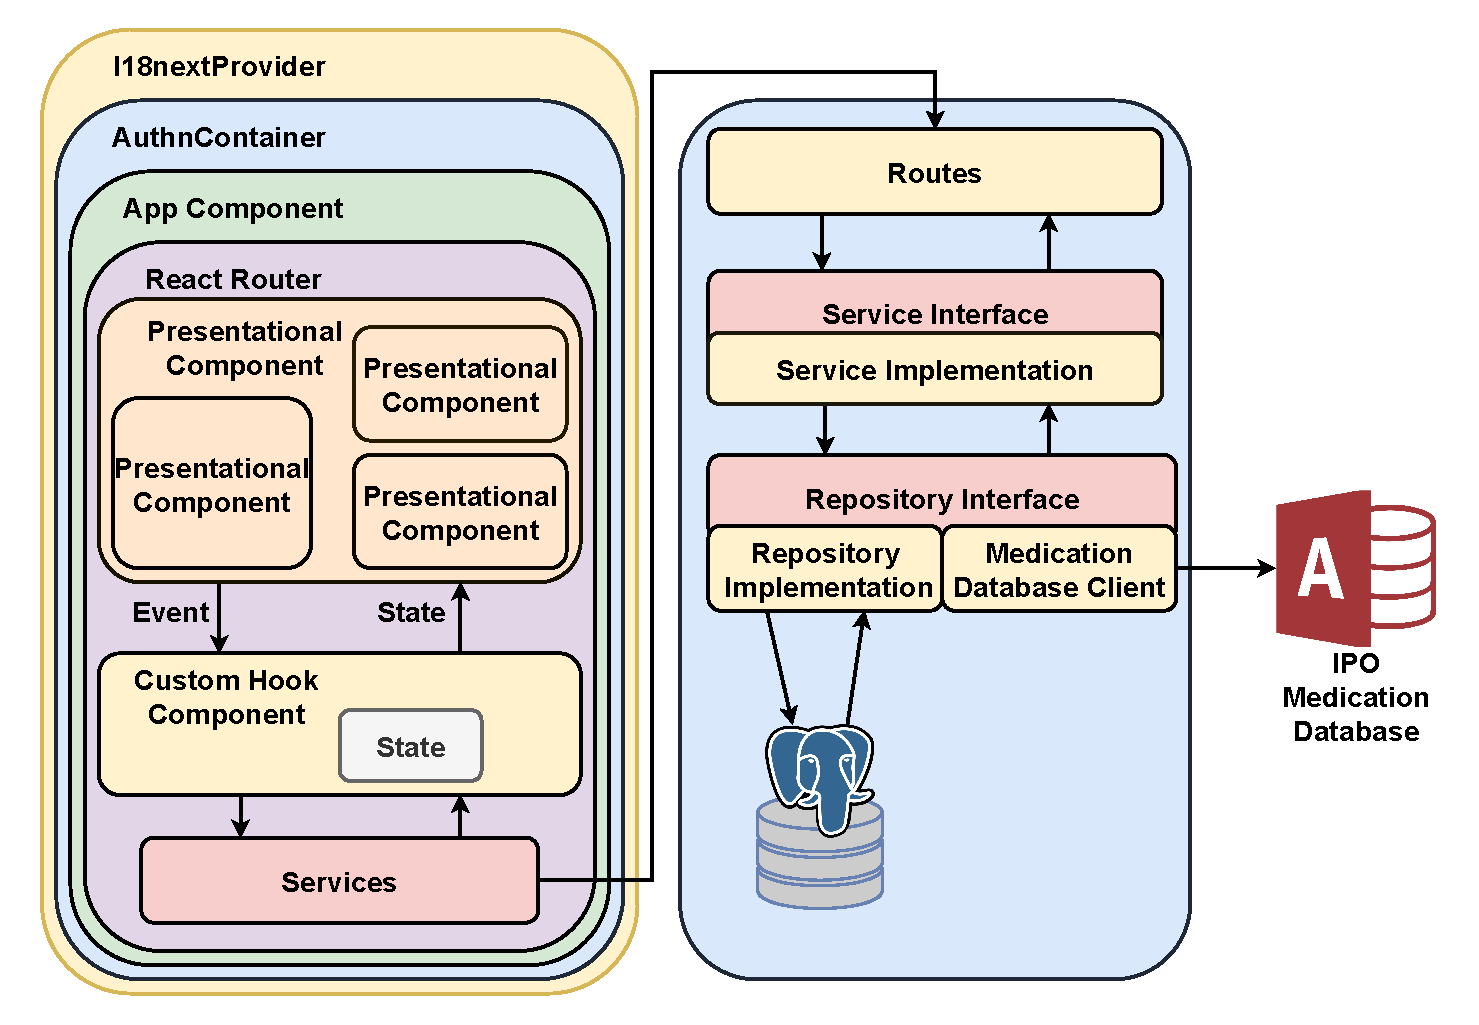
\includegraphics{./figures/Block_Diagram.pdf}}
	\end{center}
	\caption{Block Diagram of our solution.}\label{fig:Block_Diagram}
\end{figure}

\newpage
\section{Backend} \label{backend}
In this section we will describe the backend.

\subsection{Structure}

The structure for the backend application is as follows:

\begin{itemize}
 \item Program.cs: the entry point of the application;
 \item domain: contains all the domain classes;
 \item repositories: contains the backend repositories that communicate with the postgreSQL database;
 \begin{itemize}
 	\item sql: the methods to perform the requests;
 	\item entities: contains the entities outlined in chapter \ref{cap:data_model}.
 \end{itemize}
 \item services: contains all the services that, validate and manipulate data, that is received or sent to the routes and repository layer;
 \item routes: contains all the routes of the API which call the adequate service.
 \item utils: contains auxiliary classes and methods.
\end{itemize}

\subsection{Program.cs}

As mentioned before since we're creating a Minimal API, similar to apis created with Express.JS, and, as such, server creation is streamlined and the application's functionality is based on middlewares and routing.

The .NET framework makes use of a dependency injection container, aka the service container. As with the Spring Framework, dependencies can have various lifetimes, which in the .NET framework are as follows:
\begin{itemize}
	\item Transient: the dependency is created when needed and disposed thereafter;
	\item Scoped: the dependency is created and maintained in a per request basis;
	\item Singleton: once the dependency is created it's maintained throughout the application's lifetime. 
\end{itemize}
Beyond this, the framework also makes use of the builder pattern, meaning to build a web application we first instantiate a builder, i.e. a class that "knows" how to build a web application, and then supply the needed middlewares to build it, with the desired lifetime.
The aforementioned middlewares, which refer to the services and repositories, are registered as services in the container. In our application these services were registered with the Scoped scope, as follows:

\begin{lstlisting}[style=sharpc, caption=Adding middlewares using dependency injection and inversion of control]
	builder.Services.AddScoped<IUsersService, UsersService>();
	builder.Services.AddScoped<IFormService, FormService>();
	builder.Services.AddScoped<ITermsService, TermsService>();
	builder.Services.AddScoped<IMedicationsService, MedicationsService>();
	builder.Services.AddScoped<IManualService, ManualService>();


	builder.Services.AddScoped<IRepository, Repository>();
\end{lstlisting}

Using this registration method, for example, when a dependency of type IUsersService is needed, the service container creates a UsersService object to fufill that dependency, hence the inversion of control.

To allow for cross-origin resource sharing, i.e. to allow the frontend client to access the resources in the backend, we also had to create CORS policy, as follows:

\begin{lstlisting}[style=sharpc, caption={Configuring CORS Policy in ASP.NET Core: Allowing Specific Origin with Full Access Control.}]
builder.Services.AddCors(options =>
{
	options.AddPolicy("MyCorsPolicy",
	policy =>
	{
		policy.WithOrigins("http://localhost:8000")
		.AllowAnyHeader()
		.AllowAnyMethod()
		.AllowCredentials();
	});
});
\end{lstlisting}

Notice that request originating from port 8000 of the localhost ip can have any type of header, any HTTP method and can include credentials, such as cookies.
\newpage
\subsubsection{Authentication JWT}

Our platform uses JSON Web Tokens, \textbf{JWT} \cite{rfc7519}, to represent user claims.
These token's issuer, audience and key, refered to as jwtIssuer, jwtAudience and jwtKey in listing \ref{authentication} below, are stored in the appsettings.json file.

\begin{lstlisting}[style=sharpc, caption={Custom JWT Authentication Middleware in ASP.NET Core: Handling Unauthorized Access with Detailed Problem Responses.}, label={authentication}] 
builder.Services.AddAuthentication(x =>
{
	x.DefaultAuthenticateScheme = JwtBearerDefaults.AuthenticationScheme;
	x.DefaultChallengeScheme = JwtBearerDefaults.AuthenticationScheme;
}).AddJwtBearer(options =>
{
	options.Events = new JwtBearerEvents
	{
		...
		OnChallenge = context =>
		{
			context.HandleResponse();
			
			context.Response.ContentType = "application/problem+json";
			context.Response.StatusCode = StatusCodes.Status401Unauthorized;
			var problemDetails = new
			{
				type = "https://localhost:8000/errors/unauthorized",
				title = "Unauthorized",
				detail = "You are not authorized to access this resource. Please provide valid credentials.",
				status = StatusCodes.Status401Unauthorized
			};
			var problemJson = JsonSerializer.Serialize(problemDetails);
			return context.Response.WriteAsync(problemJson);
		}
	};
	options.SaveToken = true;
	options.TokenValidationParameters = new TokenValidationParameters
	{
		ValidateIssuer = true,
		ValidateAudience = true,
		ValidateLifetime = true,
		ValidateIssuerSigningKey = true,
		ValidIssuer = jwtIssuer,
		ValidAudience = jwtAudience,
		IssuerSigningKey = new SymmetricSecurityKey(Encoding.UTF8.GetBytes(jwtKey))
	};
});
\end{lstlisting}

Notice that in case the \textbf{JWT} isn't valid the default behavior of responding with a 401 status code and an empty body is suppressed by "context.HandleResponse()" and instead a Problem response is sent with more details.


%Beyond these, we also used an ElasticClient, however in this service registration, we use a different pattern, instead of using a type and implementation, only the latter was used, this method doesn't allow for multiple implementation, but since there was no need to mock the elastic search database, this feature wasn't needed.
%
%\begin{lstlisting}[style=sharpc]
%var nodePool = new SingleNodePool(new Uri("http://localhost:9200"));
%var settings = new ElasticsearchClientSettings(
% nodePool,
% sourceSerializer: (_, settings) =>
%  {
%    return new DefaultSourceSerializer(settings, options =>
%      {
%        options.Converters.Add(new AnswerConverter());
%        options.Converters.Add(new ConditionConverter());
%      });
%  });
%builder.Services.AddSingleton(new ElasticsearchClient(settings));
%\end{lstlisting}
%
%According to the Elastic Search documentation, as long as the client instance is a singleton, our application database is thread safe.
\newpage
\subsection{Repositories}

The Repository layer acts as a vital intermediary for data access within the application. It ensures the database and service layer remain independent from one another. This separation allows the service layer to access data without being tightly coupled to the database, facilitating easy database switching by merely replacing this module.

By defining a well-known interface contract, we can abstract the implementation details.

Utilizing a transaction manager in the service layer enables our solution to handle multiple concurrent accesses across various resources and provides rollback capabilities for effective error handling.

%The main idea in the repositories is to allow for CRUD operations, ie create users/forms, read users/forms, update users/forms and delete users/forms, on data that is or will be stored in an Elastic Search database. As such the repositories have a dependency on the ElasticsearchClient mentioned before, and they'll use the same client but target different indexes.

\subsubsection{Form Repository}

The form repository is responsible for the Form, Submission, Review, Inconsistency entities.

And this repository will have the following methods:

\begin{lstlisting}[style=sharpc]
public interface IFormRepository
{
	public Task<Form> GetForm();
	
	public Task<Form?> GetFormWithVersion(int version);
	
	public Task<Form> EditForm(Form form);
	
	public Task<bool> SubmitForm(Submission submission);
	
	public Task<List<Submission>?> GetPendingSubmissions();
	
	public Task<Submission> GetSubmission(int nic);
	
	public Task<Submission?> GetSubmissionById(int id);
	
	public Task<Submission?> GetLatestPendingSubmissionByUser(int userNic);
	
	public Task<(List<SubmissionHistoryDto>? Submissions, bool HasMoreSubmissions)> GetSubmissionHistoryByNic(int nic, int limit, int skip);
	
	public Task<Inconsistencies> GetInconsistencies();
	
	public Task<bool> LockSubmission(int submissionId, int doctorId);
	
	public Task<bool> UnlockSubmission(int submissionId, int doctorId);
	
	public Task<List<SubmissionLock>> GetExpiredLocks(TimeSpan timeout);
	
	public Task<bool> SubmissionExists(int id);
	
	public Task<Review> AddReview(Review review);
	
	public Task<bool> AddNote(Note note);
	
	public Task<bool> EditInconsistencies(Inconsistencies inconsistencies);
}
\end{lstlisting}

\subsubsection{User Repository}

The user repository will be responsible for the User, UserAccountStatus and UserSuspension entities

And this repository will have the following methods:
\begin{lstlisting}[style=sharpc]
public interface IUsersRepository
{
	public Task<bool> AddUser(User user);
	
	public Task<List<User>?> GetUsers();
	
	public Task<User?> GetUserByNic(int nic);
	
	public Task<Boolean> DeleteUser(int nic);
	
	public Task<UserAccountStatus?> GetUserAccountStatus(int userNic);
	
	public Task<Boolean> UpdateUserAccountStatus(UserAccountStatus userAccountStatus);
	
	public Task<bool> AddSuspension(UserSuspension suspension);
	public Task<bool> UpdateSuspension(UserSuspension suspension);
	public Task<UserSuspension?> GetSuspension(int userNic);
	public Task<bool> DeleteSuspension(int userNic);
	
}
\end{lstlisting}

\newpage

\subsection{Services}
Each service is responsible for managing a certain group of requests, i.e. the logic to fulfill a request to the /users endpoint will be in the user services. Each service as a dependency on their corresponding repository, which is handled by the service container.

The methods within each service will reflect the possible actions outlined in Chapter ~\ref{cap:problem_description}'s section on uses cases.


\subsubsection{User Service}

\begin{lstlisting}[style=sharpc]
public interface IUsersService
{
	public Task<Result<Token, Problem>> CreateToken(int nic, string password);
		
	public Task<Result<UserExternalInfo, Problem>> CreateUser(int nic, string name, string password, Role role);
		
	public Task<Result<List<UserExternalInfo>, Problem>> GetUsers(string token);
		
	public Task<Result<Boolean, Problem>> DeleteUser(int nic);
		
	public Task<Result<UserAccountStatus?, Problem>> GetUserAccountStatus(int userNic);
		
	public Task<Result<Boolean, Problem>> UpdateUserAccountStatus(UserAccountStatus userAccountStatus);
		
	public Task<Result<UserWithNameExternalInfo?, Problem>> CheckNicExistence(int nic);
		
	public Task<Result<bool, Problem>> AddSuspension(UserSuspensionRequest suspension);
		
	public Task<Result<bool, Problem>> UpdateSuspension(UserSuspension suspension);
		
	public Task<Result<UserSuspension?, Problem>> GetSuspension(int userNic);
		
	public Task<Result<bool, Problem>> DeleteSuspension(int userNic);
}
\end{lstlisting}

\newpage

\subsubsection{Terms Service}

\begin{lstlisting}[style=sharpc]
public interface ITermsService
{
	public Task<Result<List<Terms>, Problem>> GetTerms();
	public Task<Result<Terms, Problem>> GetActiveTerms();
	public Task<Result<bool, Problem>> SubmitTerms(Terms terms);
	
	public Task<Result<bool, Problem>> UpdateTerms(int termId, int updatedBy, string newContent);
	
	public Task<Result<List<TermsChangeLog>?, Problem>> GetTermsChangeLog(int termId);
}
\end{lstlisting}


\subsubsection{Form Service}

\begin{lstlisting}[style=sharpc]
public interface IFormService
{
	public Task<Result<GetFormOutputModel, Problem>> GetForm();
	
	public Task<Result<GetFormWithVersionOutputModel, Problem>> GetFormWithVersion(int version);
	
	public Task<Result<Form, Problem>> EditForm(List<QuestionGroupModel> groups, List<RuleModel> rules, User user);
	
	public Task<Result<SubmitFormOutputModel, Problem>> SubmitForm(Dictionary<string,IAnswer> answers, int nic, int formVersion);
	
	public Task<Result<Submission, Problem>> GetSubmission(int id);
	
	public Task<Result<bool, Problem>> LockSubmission(int submissionId, int doctorId);
	
	public Task<Result<bool, Problem>> UnlockSubmission(int submissionId, int doctorId);
	
	public Task UnlockExpiredSubmissions(TimeSpan lockTimeout);
	
	public Task<Result<Review, Problem>> ReviewForm(int submissionId, int doctorNic, string status, string? finalNote, List<NoteModel>? noteModels = null);
	
	public Task<Result<List<Submission>, Problem>> GetPendingSubmissions();
	
	public Task<Result<Inconsistencies, Problem>> GetInconsistencies();
	
	public Task<Result<Submission?, Problem>> GetPendingSubmissionsByUserNic(int userNic);
	
	public Task<Result<SubmissionHistoryOutputModel, Problem>> GetSubmissionHistoryByNic(int nic, int limit, int skip);
	
	public Task<Result<bool, Problem>> EditInconsistencies(Inconsistencies inconsistencies);
}
\end{lstlisting}


\subsubsection{Manual Service}

\begin{lstlisting}[style=sharpc]
public interface IManualService
{
	public Task<Result<List<ManualInformation>, Problem>> GetManualInformation(string productName);
}
\end{lstlisting}


\subsubsection{Medication Service}

\begin{lstlisting}[style=sharpc]
public interface IMedicationsService
{
	Task<Result<List<string>, Problem>> SearchMedications(string query);
}
\end{lstlisting}

\newpage

\subsection{Routes}

\subsubsection{User Routes}
The available endpoints, HTTP method and corresponding operation for all the user routes are available in Table ~\ref{tab:user_endpoints}. 

\begin{table}[h!]
	\begin{center}
		\begin{tabular}{l|c|l} 
			\textbf{Endpoint} & \textbf{HTTP Method} & \textbf{Description} \\
			\hline
			/users & POST & \makecell{Creates a new user} \\
			\hline
			/users & GET & \makecell{Retrieves all users} \\
			\hline
			/users/\{nic\} & GET & \makecell{Checks the existence of a user with the specified NIC}\\
			\hline
			/users/\{nic\} & DELETE & \makecell{Deletes the user with the specified NIC} \\
			\hline
			/users/login & POST & \makecell{Creates a new access token} \\
			\hline
			/users/status/\{nic\} & GET & \makecell{Retrieves the status of the user account\\ with the specified NIC} \\
			\hline
			/update-status & POST & \makecell{Updates the status of a user account} \\
			\hline
			/users/suspension & POST & \makecell{Adds a new suspension} \\
			\hline
			/users/suspension/update & POST & \makecell{Updates an existing suspension} \\
			\hline
			/users/suspension/\{nic\} & GET & \makecell{Retrieves the suspension details for the specified NIC} \\
			\hline
			/users/suspension/\{nic\} & DELETE & \makecell{Deletes the suspension for the specified NIC} \\
		\end{tabular}
		
		\caption{API endpoints related to the user}\label{tab:user_endpoints}
	\end{center}
\end{table}

\subsubsection{Form Routes}
The available endpoints, HTTP method and corresponding operation for all the form routes are available in Table ~\ref{tab:form_endpoints}. 
	
\begin{table}[h!]
	\begin{center}
		\begin{tabular}{l|c|l} 
			\textbf{Endpoint} & \textbf{HTTP Method} & \textbf{Description} \\
			\hline
			/forms/structure & GET & \makecell{Retrieves the form structure} \\
			\hline
			/forms/structure & PUT & \makecell{Edits the form structure} \\
			\hline
			/forms/structure/\{version:int\} & GET & \makecell{Retrieves the form structure \\ for the specified version} \\
			\hline
			/forms/submissions & GET & \makecell{Retrieves pending submissions} \\
			\hline
			/forms/submissions/\{nic:int\} & POST & \makecell{Submits a form} \\
			\hline
			/forms/submissions/\{nic:int\} & GET & \makecell{Retrieves a pending submission \\ for the specified NIC} \\
			\hline
			/forms/submissions/history/\{nic:int\} & GET & \makecell{Retrieves submission history \\ for the specified NIC} \\
			\hline
			/forms/submissions/\{submissionId:int\}/lock & POST & \makecell{Locks a submission} \\
			\hline
			/forms/submissions/\{submissionId:int\}/unlock & POST & \makecell{Unlocks a submission} \\
			\hline
			/forms/inconsistencies & GET & \makecell{Retrieves inconsistencies} \\
			\hline
			/forms/inconsistencies & PUT & \makecell{Edits inconsistencies} \\
			\hline
			/forms/review/\{submissionId:int\} & POST & \makecell{Reviews a form submission} \\
			\hline
			/forms/notifications & GET & \makecell{Sets up server-sent \\ event notifications} \\
		\end{tabular}
		
		\caption{API endpoints related to the form}\label{tab:form_endpoints}
	\end{center}
\end{table}

\subsubsection{Terms Routes}
\begin{table}[h!]
	\begin{center}
		\begin{tabular}{l|c|l} 
			\textbf{Endpoint} & \textbf{HTTP Method} & \textbf{Description} \\
			\hline
			/terms & GET & \makecell{Retrieves all the terms} \\
			\hline
			/terms/active & GET & \makecell{Retrieves the active terms} \\
			\hline
			/terms & POST & \makecell{Submits terms} \\
			\hline
			/terms/\{termsId:int\} & PUT & \makecell{Updates terms with the specified termsId} \\
			\hline
			/terms/change-log/\{termsId:int\} & GET & \makecell{Gets the change-logs\\ for the terms with  specified termsId} \\
		\end{tabular}
		
		\caption{API endpoints related to the form}\label{tab:term_endpoints}
	\end{center}
\end{table}

\subsubsection{Medication and Manual Routes}
\begin{table}[h!]
	\begin{center}
		\begin{tabular}{l|c|l} 
			\textbf{Endpoint} & \textbf{HTTP Method} & \textbf{Description} \\
			\hline
			/medications/search & GET & \makecell{Retrieves medication list according to a query string} \\
			\hline
			/manual/\{product:string\} & GET & \makecell{Retrieves the blood donation information relevant to the specific product} \\
		\end{tabular}
		
		\caption{API endpoints related to the form}\label{tab:medication_manual_endpoints}
	\end{center}
\end{table}

\newpage

\section{Frontend} \label{frontend}

The frontend application is tasked with data visualization and user interaction. The objective is for the application to provide an intuitive interface for the various users to be able to fulfill the set use cases outlined in section ~\ref{sec:use_cases}.

The frontend is implemented in Typescript and React, and makes use of JSON-Rules-Engine to enforce the form's rules, for further information about these technologies refer to ~\ref{sec:frontend_tech}.

\subsection{Structure}

The frontend structure is as follows:

\begin{itemize}
	\item src: contains the source code of the application;
	\item public: contains the static files of the application;
	\item package.json:  package.json;
	\item tsconfig.json: contains the TypeScript configuration;
	\item routes: contains all the routes of the API which call the adequate service.
	\item webpack.config.js:  contains the Webpack configuration.
\end{itemize}

The src folder is then subdivided into multiple folders/files, each being responsible for a different functionality of the application:

\begin{itemize}
	\item components: contains the components of the pages;
	\item domain: contains the domain objects;
	\item pages:  contains the application's pages, each containing various components;
	\item services: contains the services that communicate with the backend application;
	\item session: contains the code needed to maintain a user session.
	\item utils:  contains general utility functions.
\end{itemize}

It should be noted that, folders within the components folder may contain further utils, containing utility functions that are specially pertinent for that component and shouldn't necessarily be in the general utils. 

Furthermore, besides the aforementioned folders, the src folder also contains an index.tsx and App.tsx files. The index.tsx file is the entry point for the application meanwhile the App.tsx is the main component of the React application.


\section{Services}

The frontend services are responsible for communicating with the backend application and, as such, each frontend service as a backend counterpart.

To facilitate this communication we used the Fetch API \cite{Fetch_API}, which enables asynchronous resource requests by returning a promise that resolves to a response for that request.

To expedite, and reduce the code for, the api resource requests we created a fetchAPI function that accepts the request parameters and return a promise that will resolve to the requests response, this function can also handle errors if the response's status code isn't in the 200 family.

To further abstract the api calls,  the fetchAPI function was encapsulated within functions that represent specific HTTP methods, such as GET, POST, PUT and DELETE.

\newpage

\section{Components}

A simplified view of the component tree is presented in Figure ~\ref{fig:reactComponentTree}, in this chapter we'll mainly focus on the I18nextProvider which manages the language preferences of the user, AuthnContainer, which manages the session information, the Form, Backoffice, EditFormPage, EditTermsPage and Editor which are presentational components and the useNewForm, useEditFormPage, useEditTerms which are custom hooks.

\begin{figure}[H]
	\begin{center}
		\resizebox{130mm}{!}{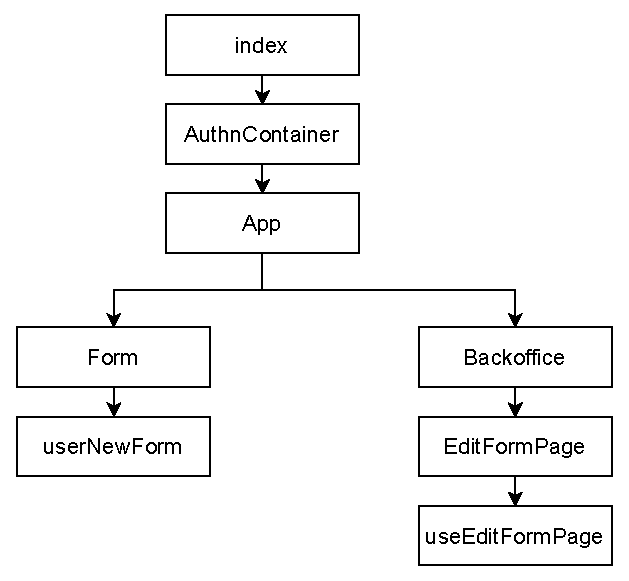
\includegraphics{./figures/reactComponentTree.pdf}}
	\end{center}
	\caption{Simplified React Component Tree.}\label{fig:reactComponentTree}
\end{figure}

\subsection{I18nextProvider}

The I18nextProvider component is part of the i18next library ecosystem, which is used for internationalization (i18n) in JavaScript applications. The purpose of the I18nextProvider component is to integrate i18next into React applications by providing the i18n instance to the component tree.

By accessing the i18n instance, we can set the desired language for the application. This is useful for both the frontend and to request certain resources from the backend, i.e. requesting the resource with the user's language preferences, or default to a certain resource if that isn't available.


\subsection{AuthnContainer}
The AuthnContainer component plays a crucial role in enabling user authentication and consequent storage of the authentication information within the application state.

To do so it uses the React Context API \cite{React_Context_API}, which allows to pass data trough the component tree without having to pass props down manually at every level, thus enabling seamless data sharing between components.

The Session type describe a user's session, i.e. their name and nic. The SessionManager type acts as a wrapper, containing both the session and the methods to manage it, i.e. set a session and delete it.

The AuthContainer component wraps it's child components within it's LoggedInContext.Provider, providing the session manager instance and it's methods as the context value, making the authentication information available throughout the component tree.

\subsection{Form}
The Form component is the central component of the application serving as the form page. It leverages the useNewForm hook, which is responsible for retrieving the form structure from the backend and manage it within the application state.

As the user answers the form's the JSON-Rules-Engine is run and, according to the rules in the form, events are triggered, showing or hiding questions, allowing the user to answer the next group of questions or reviewing their answers.

\subsection{EditFormPage}
The EditFormPage component acts a an outlet for the backoffice component page. It leverages the useEditFormPage hook to retrieve the form structure from the backend and manage it's state.

As the user edit's the form's structure the changes are reflected in the hook's state, which is specially difficult given that a question can be a parent, i.e. it's answer causes another question to appear, and a child, i.e. it appears as a result of another question's answer.

To solve this issue the hook can reassign questions upon deletion, by finding the group with the parent question and setting the show condition of it's child question as undefined, which means they're automatically shown.

\subsection{EditTermsPage}

The EditTermsPage component acts as an outlet for the backoffice component page. It provides an interface for editing the terms and conditions. This component leverages the Editor component, which integrates the Jodit WYSIWYG editor, offering a rich text editing experience. The state management is handled using the useEditTerms custom hook, which ensures seamless interaction with the backend.
The content of the editor is stored as HTML allowing for flexible presentation and formatting when displayed to end-users.


\newpage

\section{Navigation}

This chapter features a navigation graph, presented in Figure ~\ref{fig:userNavigation}, that describes the UI flow of our platform.
The primary entry point for all users is the Home page, from which navigation diverges based on the user's login status and role.
With admins being able to navigate throughout the platform, while doctors lack backoffice access and finally donors only having access to the terms and form page.

\begin{figure}[H]
	\begin{center}
		\resizebox{150mm}{!}{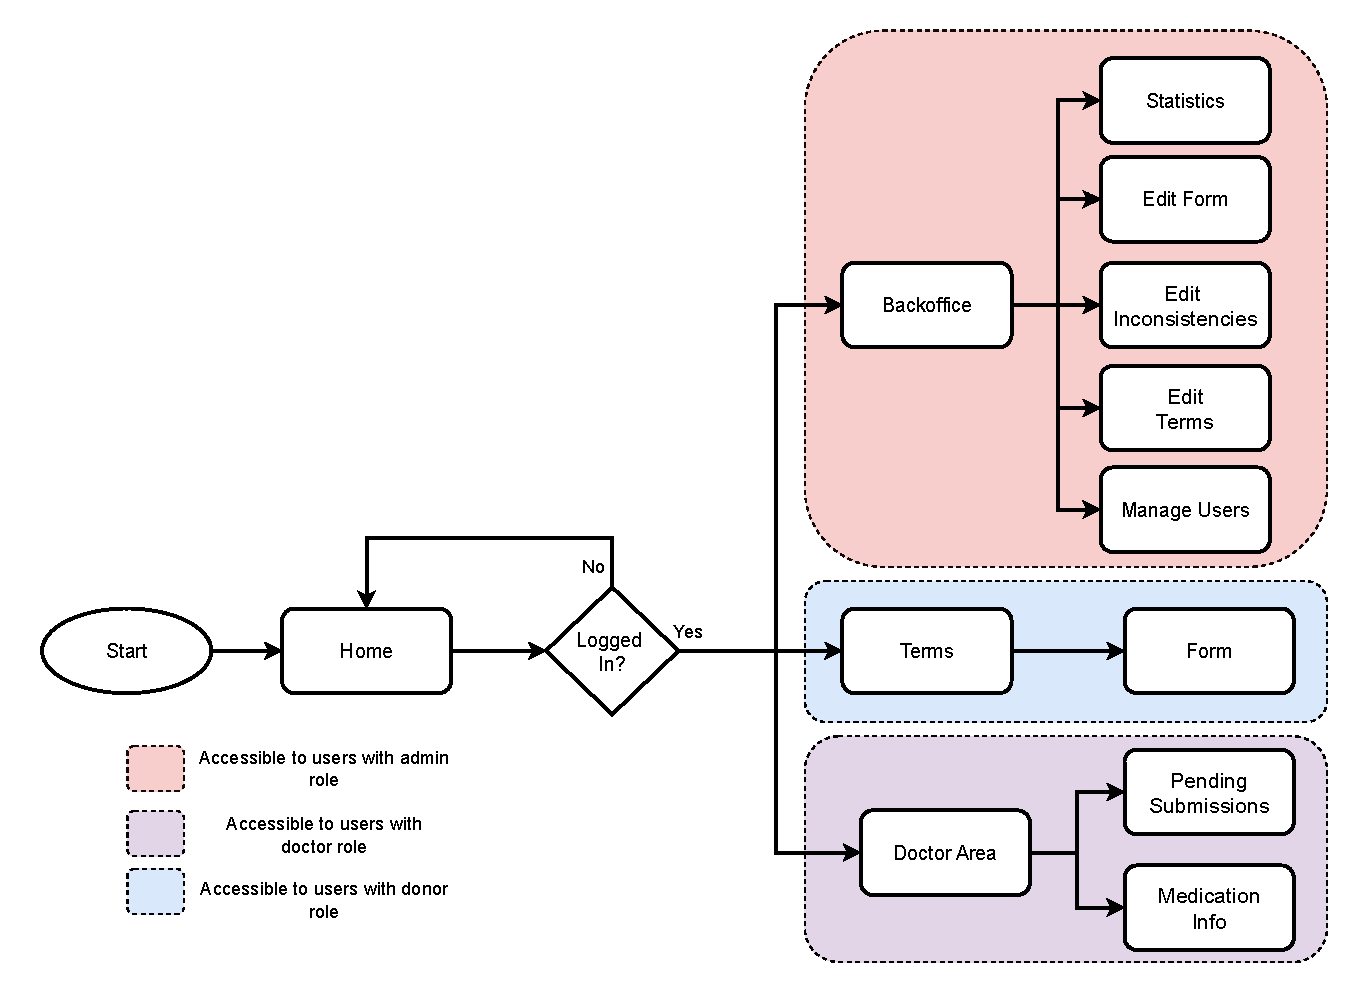
\includegraphics{./figures/userNavigation.pdf}}
	\end{center}
	\caption{UI navigation.}\label{fig:userNavigation}
\end{figure}










